% !TEX encoding = UTF-8 Unicode
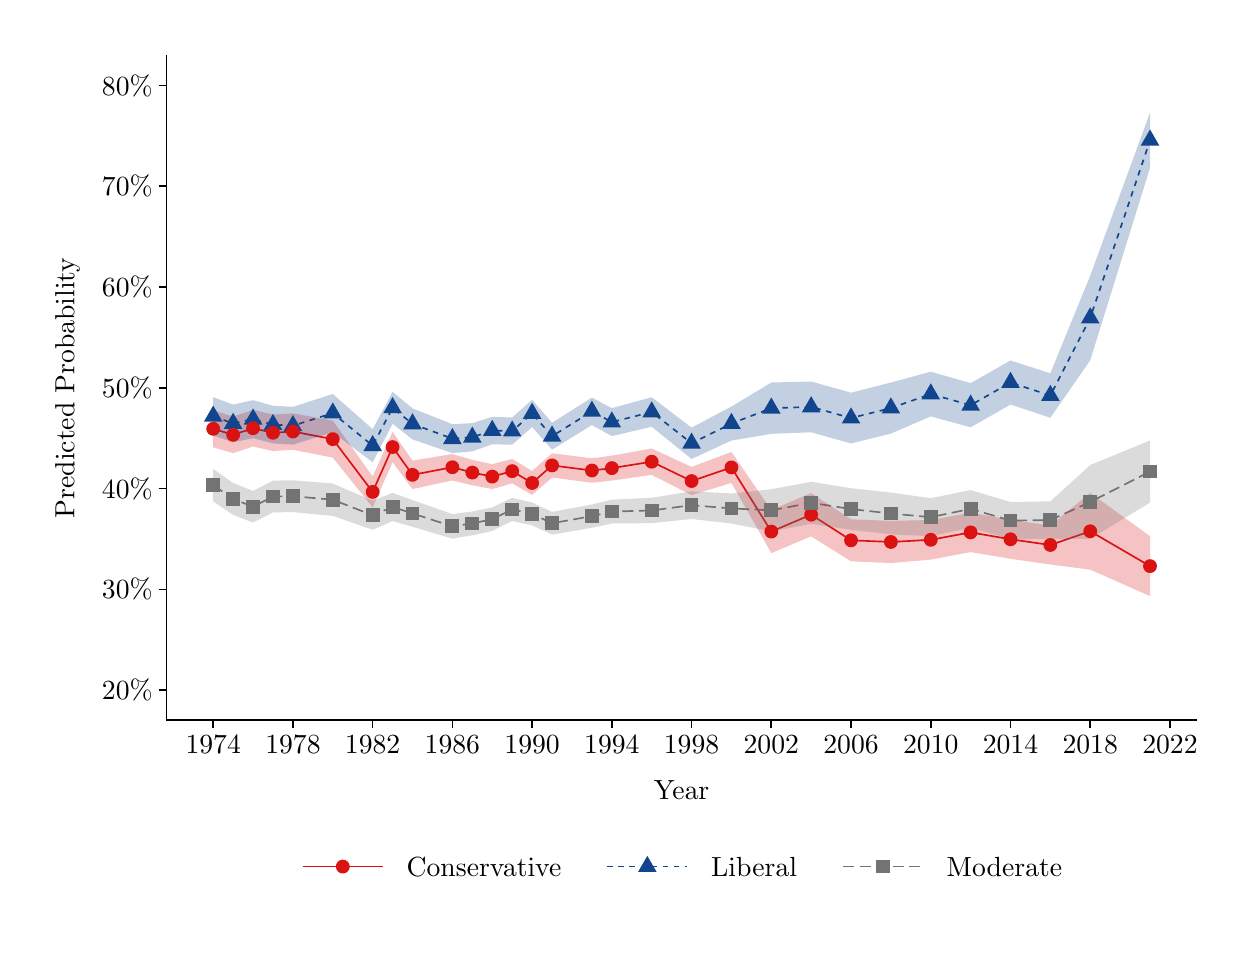
\begin{tikzpicture}[x=1pt,y=1pt]
\definecolor{fillColor}{RGB}{255,255,255}
\path[use as bounding box,fill=fillColor,fill opacity=0.00] (0,0) rectangle (432.48,324.36);
\begin{scope}
\path[clip] (  0.00,  0.00) rectangle (432.48,324.36);
\definecolor{fillColor}{RGB}{255,255,255}

\path[fill=fillColor] ( -0.00,  0.00) rectangle (432.48,324.36);
\end{scope}
\begin{scope}
\path[clip] ( 50.11, 74.07) rectangle (422.48,314.36);
\definecolor{fillColor}{RGB}{255,255,255}

\path[fill=fillColor] ( 50.11, 74.07) rectangle (422.48,314.36);
\definecolor{drawColor}{RGB}{218,18,18}

\path[draw=drawColor,line width= 0.6pt,line join=round] ( 67.04,179.41) --
	( 74.24,177.24) --
	( 81.44,179.62) --
	( 88.64,177.96) --
	( 95.85,178.43) --
	(110.25,175.67) --
	(124.66,156.61) --
	(131.86,172.82) --
	(139.06,162.77) --
	(153.47,165.52) --
	(160.67,163.59) --
	(167.87,162.14) --
	(175.07,164.11) --
	(182.28,159.83) --
	(189.48,166.18) --
	(203.88,164.34) --
	(211.09,165.20) --
	(225.49,167.52) --
	(239.90,160.53) --
	(254.30,165.45) --
	(268.71,142.28) --
	(283.11,148.38) --
	(297.52,139.12) --
	(311.92,138.52) --
	(326.33,139.30) --
	(340.73,141.98) --
	(355.14,139.49) --
	(369.54,137.43) --
	(383.95,142.39) --
	(405.56,129.79);
\definecolor{drawColor}{RGB}{17,70,143}

\path[draw=drawColor,line width= 0.6pt,dash pattern=on 2pt off 2pt ,line join=round] ( 67.04,183.94) --
	( 74.24,181.34) --
	( 81.44,182.89) --
	( 88.64,180.93) --
	( 95.85,180.52) --
	(110.25,185.08) --
	(124.66,173.30) --
	(131.86,187.00) --
	(139.06,181.17) --
	(153.47,175.85) --
	(160.67,176.35) --
	(167.87,178.79) --
	(175.07,178.57) --
	(182.28,184.96) --
	(189.48,176.73) --
	(203.88,185.73) --
	(211.09,181.83) --
	(225.49,185.48) --
	(239.90,174.17) --
	(254.30,181.31) --
	(268.71,186.86) --
	(283.11,187.32) --
	(297.52,183.29) --
	(311.92,186.90) --
	(326.33,191.97) --
	(340.73,187.93) --
	(355.14,196.13) --
	(369.54,191.43) --
	(383.95,219.45) --
	(405.56,283.68);
\definecolor{drawColor}{gray}{0.45}

\path[draw=drawColor,line width= 0.6pt,dash pattern=on 4pt off 2pt ,line join=round] ( 67.04,159.04) --
	( 74.24,154.05) --
	( 81.44,151.25) --
	( 88.64,154.94) --
	( 95.85,155.05) --
	(110.25,153.79) --
	(124.66,148.17) --
	(131.86,151.17) --
	(139.06,148.82) --
	(153.47,144.16) --
	(160.67,145.22) --
	(167.87,146.74) --
	(175.07,150.28) --
	(182.28,148.63) --
	(189.48,145.29) --
	(203.88,147.85) --
	(211.09,149.49) --
	(225.49,149.91) --
	(239.90,151.80) --
	(254.30,150.63) --
	(268.71,149.95) --
	(283.11,152.67) --
	(297.52,150.41) --
	(311.92,148.80) --
	(326.33,147.47) --
	(340.73,150.48) --
	(355.14,146.25) --
	(369.54,146.43) --
	(383.95,152.96) --
	(405.56,163.97);
\definecolor{fillColor}{RGB}{218,18,18}

\path[fill=fillColor,fill opacity=0.25] ( 67.04,186.11) --
	( 74.24,183.86) --
	( 81.44,186.22) --
	( 88.64,184.55) --
	( 95.85,185.02) --
	(110.25,182.36) --
	(124.66,162.18) --
	(131.86,178.29) --
	(139.06,167.91) --
	(153.47,170.29) --
	(160.67,168.19) --
	(167.87,166.64) --
	(175.07,168.51) --
	(182.28,164.17) --
	(189.48,170.55) --
	(203.88,168.76) --
	(211.09,169.70) --
	(225.49,172.28) --
	(239.90,165.63) --
	(254.30,171.05) --
	(268.71,150.06) --
	(283.11,156.20) --
	(297.52,146.70) --
	(311.92,146.14) --
	(326.33,146.46) --
	(340.73,149.09) --
	(355.14,146.52) --
	(369.54,144.49) --
	(383.95,156.25) --
	(405.56,140.61) --
	(405.56,118.96) --
	(383.95,128.52) --
	(369.54,130.38) --
	(355.14,132.45) --
	(340.73,134.87) --
	(326.33,132.14) --
	(311.92,130.89) --
	(297.52,131.53) --
	(283.11,140.55) --
	(268.71,134.50) --
	(254.30,159.86) --
	(239.90,155.43) --
	(225.49,162.77) --
	(211.09,160.70) --
	(203.88,159.93) --
	(189.48,161.81) --
	(182.28,155.49) --
	(175.07,159.71) --
	(167.87,157.63) --
	(160.67,158.99) --
	(153.47,160.75) --
	(139.06,157.63) --
	(131.86,167.35) --
	(124.66,151.04) --
	(110.25,168.99) --
	( 95.85,171.83) --
	( 88.64,171.38) --
	( 81.44,173.01) --
	( 74.24,170.62) --
	( 67.04,172.72) --
	cycle;

\path[] ( 67.04,186.11) --
	( 74.24,183.86) --
	( 81.44,186.22) --
	( 88.64,184.55) --
	( 95.85,185.02) --
	(110.25,182.36) --
	(124.66,162.18) --
	(131.86,178.29) --
	(139.06,167.91) --
	(153.47,170.29) --
	(160.67,168.19) --
	(167.87,166.64) --
	(175.07,168.51) --
	(182.28,164.17) --
	(189.48,170.55) --
	(203.88,168.76) --
	(211.09,169.70) --
	(225.49,172.28) --
	(239.90,165.63) --
	(254.30,171.05) --
	(268.71,150.06) --
	(283.11,156.20) --
	(297.52,146.70) --
	(311.92,146.14) --
	(326.33,146.46) --
	(340.73,149.09) --
	(355.14,146.52) --
	(369.54,144.49) --
	(383.95,156.25) --
	(405.56,140.61);

\path[] (405.56,118.96) --
	(383.95,128.52) --
	(369.54,130.38) --
	(355.14,132.45) --
	(340.73,134.87) --
	(326.33,132.14) --
	(311.92,130.89) --
	(297.52,131.53) --
	(283.11,140.55) --
	(268.71,134.50) --
	(254.30,159.86) --
	(239.90,155.43) --
	(225.49,162.77) --
	(211.09,160.70) --
	(203.88,159.93) --
	(189.48,161.81) --
	(182.28,155.49) --
	(175.07,159.71) --
	(167.87,157.63) --
	(160.67,158.99) --
	(153.47,160.75) --
	(139.06,157.63) --
	(131.86,167.35) --
	(124.66,151.04) --
	(110.25,168.99) --
	( 95.85,171.83) --
	( 88.64,171.38) --
	( 81.44,173.01) --
	( 74.24,170.62) --
	( 67.04,172.72);
\definecolor{fillColor}{RGB}{17,70,143}

\path[fill=fillColor,fill opacity=0.25] ( 67.04,190.84) --
	( 74.24,188.16) --
	( 81.44,189.75) --
	( 88.64,187.74) --
	( 95.85,187.34) --
	(110.25,192.00) --
	(124.66,179.29) --
	(131.86,192.75) --
	(139.06,186.78) --
	(153.47,181.07) --
	(160.67,181.44) --
	(167.87,183.75) --
	(175.07,183.49) --
	(182.28,189.89) --
	(189.48,181.59) --
	(203.88,190.69) --
	(211.09,186.88) --
	(225.49,190.81) --
	(239.90,179.83) --
	(254.30,187.46) --
	(268.71,196.13) --
	(283.11,196.50) --
	(297.52,192.45) --
	(311.92,196.12) --
	(326.33,200.05) --
	(340.73,195.91) --
	(355.14,204.10) --
	(369.54,199.46) --
	(383.95,234.75) --
	(405.56,293.65) --
	(405.56,273.72) --
	(383.95,204.15) --
	(369.54,183.41) --
	(355.14,188.17) --
	(340.73,179.95) --
	(326.33,183.89) --
	(311.92,177.68) --
	(297.52,174.12) --
	(283.11,178.15) --
	(268.71,177.59) --
	(254.30,175.16) --
	(239.90,168.51) --
	(225.49,180.15) --
	(211.09,176.78) --
	(203.88,180.77) --
	(189.48,171.88) --
	(182.28,180.03) --
	(175.07,173.65) --
	(167.87,173.83) --
	(160.67,171.26) --
	(153.47,170.63) --
	(139.06,175.57) --
	(131.86,181.25) --
	(124.66,167.31) --
	(110.25,178.16) --
	( 95.85,173.69) --
	( 88.64,174.12) --
	( 81.44,176.03) --
	( 74.24,174.51) --
	( 67.04,177.03) --
	cycle;

\path[] ( 67.04,190.84) --
	( 74.24,188.16) --
	( 81.44,189.75) --
	( 88.64,187.74) --
	( 95.85,187.34) --
	(110.25,192.00) --
	(124.66,179.29) --
	(131.86,192.75) --
	(139.06,186.78) --
	(153.47,181.07) --
	(160.67,181.44) --
	(167.87,183.75) --
	(175.07,183.49) --
	(182.28,189.89) --
	(189.48,181.59) --
	(203.88,190.69) --
	(211.09,186.88) --
	(225.49,190.81) --
	(239.90,179.83) --
	(254.30,187.46) --
	(268.71,196.13) --
	(283.11,196.50) --
	(297.52,192.45) --
	(311.92,196.12) --
	(326.33,200.05) --
	(340.73,195.91) --
	(355.14,204.10) --
	(369.54,199.46) --
	(383.95,234.75) --
	(405.56,293.65);

\path[] (405.56,273.72) --
	(383.95,204.15) --
	(369.54,183.41) --
	(355.14,188.17) --
	(340.73,179.95) --
	(326.33,183.89) --
	(311.92,177.68) --
	(297.52,174.12) --
	(283.11,178.15) --
	(268.71,177.59) --
	(254.30,175.16) --
	(239.90,168.51) --
	(225.49,180.15) --
	(211.09,176.78) --
	(203.88,180.77) --
	(189.48,171.88) --
	(182.28,180.03) --
	(175.07,173.65) --
	(167.87,173.83) --
	(160.67,171.26) --
	(153.47,170.63) --
	(139.06,175.57) --
	(131.86,181.25) --
	(124.66,167.31) --
	(110.25,178.16) --
	( 95.85,173.69) --
	( 88.64,174.12) --
	( 81.44,176.03) --
	( 74.24,174.51) --
	( 67.04,177.03);
\definecolor{fillColor}{RGB}{115,115,115}

\path[fill=fillColor,fill opacity=0.25] ( 67.04,164.92) --
	( 74.24,159.81) --
	( 81.44,156.97) --
	( 88.64,160.68) --
	( 95.85,160.80) --
	(110.25,159.65) --
	(124.66,153.41) --
	(131.86,156.28) --
	(139.06,153.65) --
	(153.47,148.59) --
	(160.67,149.52) --
	(167.87,151.01) --
	(175.07,154.47) --
	(182.28,152.74) --
	(189.48,149.39) --
	(203.88,152.05) --
	(211.09,153.80) --
	(225.49,154.48) --
	(239.90,156.79) --
	(254.30,156.05) --
	(268.71,157.57) --
	(283.11,160.25) --
	(297.52,157.94) --
	(311.92,156.36) --
	(326.33,154.33) --
	(340.73,157.28) --
	(355.14,152.96) --
	(369.54,153.20) --
	(383.95,166.30) --
	(405.56,175.20) --
	(405.56,152.74) --
	(383.95,139.63) --
	(369.54,139.65) --
	(355.14,139.55) --
	(340.73,143.67) --
	(326.33,140.61) --
	(311.92,141.25) --
	(297.52,142.89) --
	(283.11,145.09) --
	(268.71,142.32) --
	(254.30,145.20) --
	(239.90,146.81) --
	(225.49,145.33) --
	(211.09,145.19) --
	(203.88,143.64) --
	(189.48,141.19) --
	(182.28,144.53) --
	(175.07,146.08) --
	(167.87,142.48) --
	(160.67,140.92) --
	(153.47,139.72) --
	(139.06,144.00) --
	(131.86,146.07) --
	(124.66,142.94) --
	(110.25,147.93) --
	( 95.85,149.30) --
	( 88.64,149.21) --
	( 81.44,145.53) --
	( 74.24,148.29) --
	( 67.04,153.17) --
	cycle;

\path[] ( 67.04,164.92) --
	( 74.24,159.81) --
	( 81.44,156.97) --
	( 88.64,160.68) --
	( 95.85,160.80) --
	(110.25,159.65) --
	(124.66,153.41) --
	(131.86,156.28) --
	(139.06,153.65) --
	(153.47,148.59) --
	(160.67,149.52) --
	(167.87,151.01) --
	(175.07,154.47) --
	(182.28,152.74) --
	(189.48,149.39) --
	(203.88,152.05) --
	(211.09,153.80) --
	(225.49,154.48) --
	(239.90,156.79) --
	(254.30,156.05) --
	(268.71,157.57) --
	(283.11,160.25) --
	(297.52,157.94) --
	(311.92,156.36) --
	(326.33,154.33) --
	(340.73,157.28) --
	(355.14,152.96) --
	(369.54,153.20) --
	(383.95,166.30) --
	(405.56,175.20);

\path[] (405.56,152.74) --
	(383.95,139.63) --
	(369.54,139.65) --
	(355.14,139.55) --
	(340.73,143.67) --
	(326.33,140.61) --
	(311.92,141.25) --
	(297.52,142.89) --
	(283.11,145.09) --
	(268.71,142.32) --
	(254.30,145.20) --
	(239.90,146.81) --
	(225.49,145.33) --
	(211.09,145.19) --
	(203.88,143.64) --
	(189.48,141.19) --
	(182.28,144.53) --
	(175.07,146.08) --
	(167.87,142.48) --
	(160.67,140.92) --
	(153.47,139.72) --
	(139.06,144.00) --
	(131.86,146.07) --
	(124.66,142.94) --
	(110.25,147.93) --
	( 95.85,149.30) --
	( 88.64,149.21) --
	( 81.44,145.53) --
	( 74.24,148.29) --
	( 67.04,153.17);
\definecolor{fillColor}{RGB}{17,70,143}

\path[fill=fillColor] ( 67.04,187.82) --
	( 70.40,181.99) --
	( 63.67,181.99) --
	cycle;

\path[fill=fillColor] ( 74.24,185.22) --
	( 77.60,179.39) --
	( 70.87,179.39) --
	cycle;

\path[fill=fillColor] ( 81.44,186.77) --
	( 84.80,180.95) --
	( 78.08,180.95) --
	cycle;

\path[fill=fillColor] ( 88.64,184.82) --
	( 92.01,178.99) --
	( 85.28,178.99) --
	cycle;

\path[fill=fillColor] ( 95.85,184.40) --
	( 99.21,178.58) --
	( 92.48,178.58) --
	cycle;

\path[fill=fillColor] (110.25,188.97) --
	(113.62,183.14) --
	(106.89,183.14) --
	cycle;

\path[fill=fillColor] (124.66,177.18) --
	(128.02,171.36) --
	(121.29,171.36) --
	cycle;

\path[fill=fillColor] (131.86,190.89) --
	(135.22,185.06) --
	(128.50,185.06) --
	cycle;

\path[fill=fillColor] (139.06,185.06) --
	(142.43,179.23) --
	(135.70,179.23) --
	cycle;

\path[fill=fillColor] (153.47,179.74) --
	(156.83,173.91) --
	(150.10,173.91) --
	cycle;

\path[fill=fillColor] (160.67,180.24) --
	(164.03,174.41) --
	(157.31,174.41) --
	cycle;

\path[fill=fillColor] (167.87,182.68) --
	(171.24,176.85) --
	(164.51,176.85) --
	cycle;

\path[fill=fillColor] (175.07,182.45) --
	(178.44,176.63) --
	(171.71,176.63) --
	cycle;

\path[fill=fillColor] (182.28,188.85) --
	(185.64,183.02) --
	(178.91,183.02) --
	cycle;

\path[fill=fillColor] (189.48,180.62) --
	(192.84,174.79) --
	(186.12,174.79) --
	cycle;

\path[fill=fillColor] (203.88,189.61) --
	(207.25,183.79) --
	(200.52,183.79) --
	cycle;

\path[fill=fillColor] (211.09,185.72) --
	(214.45,179.89) --
	(207.72,179.89) --
	cycle;

\path[fill=fillColor] (225.49,189.36) --
	(228.86,183.53) --
	(222.13,183.53) --
	cycle;

\path[fill=fillColor] (239.90,178.05) --
	(243.26,172.23) --
	(236.53,172.23) --
	cycle;

\path[fill=fillColor] (254.30,185.20) --
	(257.67,179.37) --
	(250.94,179.37) --
	cycle;

\path[fill=fillColor] (268.71,190.74) --
	(272.07,184.92) --
	(265.34,184.92) --
	cycle;

\path[fill=fillColor] (283.11,191.21) --
	(286.48,185.38) --
	(279.75,185.38) --
	cycle;

\path[fill=fillColor] (297.52,187.17) --
	(300.88,181.34) --
	(294.15,181.34) --
	cycle;

\path[fill=fillColor] (311.92,190.78) --
	(315.29,184.96) --
	(308.56,184.96) --
	cycle;

\path[fill=fillColor] (326.33,195.85) --
	(329.69,190.03) --
	(322.96,190.03) --
	cycle;

\path[fill=fillColor] (340.73,191.82) --
	(344.10,185.99) --
	(337.37,185.99) --
	cycle;

\path[fill=fillColor] (355.14,200.02) --
	(358.50,194.19) --
	(351.77,194.19) --
	cycle;

\path[fill=fillColor] (369.54,195.32) --
	(372.91,189.49) --
	(366.18,189.49) --
	cycle;

\path[fill=fillColor] (383.95,223.34) --
	(387.31,217.51) --
	(380.58,217.51) --
	cycle;

\path[fill=fillColor] (405.56,287.57) --
	(408.92,281.74) --
	(402.19,281.74) --
	cycle;
\definecolor{fillColor}{RGB}{218,18,18}

\path[fill=fillColor] ( 67.04,179.41) circle (  2.50);

\path[fill=fillColor] ( 74.24,177.24) circle (  2.50);

\path[fill=fillColor] ( 81.44,179.62) circle (  2.50);

\path[fill=fillColor] ( 88.64,177.96) circle (  2.50);

\path[fill=fillColor] ( 95.85,178.43) circle (  2.50);

\path[fill=fillColor] (110.25,175.67) circle (  2.50);

\path[fill=fillColor] (124.66,156.61) circle (  2.50);

\path[fill=fillColor] (131.86,172.82) circle (  2.50);

\path[fill=fillColor] (139.06,162.77) circle (  2.50);

\path[fill=fillColor] (153.47,165.52) circle (  2.50);

\path[fill=fillColor] (160.67,163.59) circle (  2.50);

\path[fill=fillColor] (167.87,162.14) circle (  2.50);

\path[fill=fillColor] (175.07,164.11) circle (  2.50);

\path[fill=fillColor] (182.28,159.83) circle (  2.50);

\path[fill=fillColor] (189.48,166.18) circle (  2.50);

\path[fill=fillColor] (203.88,164.34) circle (  2.50);

\path[fill=fillColor] (211.09,165.20) circle (  2.50);

\path[fill=fillColor] (225.49,167.52) circle (  2.50);

\path[fill=fillColor] (239.90,160.53) circle (  2.50);

\path[fill=fillColor] (254.30,165.45) circle (  2.50);

\path[fill=fillColor] (268.71,142.28) circle (  2.50);

\path[fill=fillColor] (283.11,148.38) circle (  2.50);

\path[fill=fillColor] (297.52,139.12) circle (  2.50);

\path[fill=fillColor] (311.92,138.52) circle (  2.50);

\path[fill=fillColor] (326.33,139.30) circle (  2.50);

\path[fill=fillColor] (340.73,141.98) circle (  2.50);

\path[fill=fillColor] (355.14,139.49) circle (  2.50);

\path[fill=fillColor] (369.54,137.43) circle (  2.50);

\path[fill=fillColor] (383.95,142.39) circle (  2.50);

\path[fill=fillColor] (405.56,129.79) circle (  2.50);
\definecolor{fillColor}{gray}{0.45}

\path[fill=fillColor] ( 64.54,156.54) --
	( 69.53,156.54) --
	( 69.53,161.54) --
	( 64.54,161.54) --
	cycle;

\path[fill=fillColor] ( 71.74,151.55) --
	( 76.74,151.55) --
	( 76.74,156.55) --
	( 71.74,156.55) --
	cycle;

\path[fill=fillColor] ( 78.94,148.75) --
	( 83.94,148.75) --
	( 83.94,153.75) --
	( 78.94,153.75) --
	cycle;

\path[fill=fillColor] ( 86.15,152.45) --
	( 91.14,152.45) --
	( 91.14,157.44) --
	( 86.15,157.44) --
	cycle;

\path[fill=fillColor] ( 93.35,152.55) --
	( 98.34,152.55) --
	( 98.34,157.55) --
	( 93.35,157.55) --
	cycle;

\path[fill=fillColor] (107.75,151.29) --
	(112.75,151.29) --
	(112.75,156.29) --
	(107.75,156.29) --
	cycle;

\path[fill=fillColor] (122.16,145.67) --
	(127.15,145.67) --
	(127.15,150.67) --
	(122.16,150.67) --
	cycle;

\path[fill=fillColor] (129.36,148.68) --
	(134.36,148.68) --
	(134.36,153.67) --
	(129.36,153.67) --
	cycle;

\path[fill=fillColor] (136.56,146.33) --
	(141.56,146.33) --
	(141.56,151.32) --
	(136.56,151.32) --
	cycle;

\path[fill=fillColor] (150.97,141.66) --
	(155.96,141.66) --
	(155.96,146.65) --
	(150.97,146.65) --
	cycle;

\path[fill=fillColor] (158.17,142.72) --
	(163.17,142.72) --
	(163.17,147.71) --
	(158.17,147.71) --
	cycle;

\path[fill=fillColor] (165.37,144.25) --
	(170.37,144.25) --
	(170.37,149.24) --
	(165.37,149.24) --
	cycle;

\path[fill=fillColor] (172.58,147.78) --
	(177.57,147.78) --
	(177.57,152.77) --
	(172.58,152.77) --
	cycle;

\path[fill=fillColor] (179.78,146.13) --
	(184.77,146.13) --
	(184.77,151.13) --
	(179.78,151.13) --
	cycle;

\path[fill=fillColor] (186.98,142.79) --
	(191.98,142.79) --
	(191.98,147.78) --
	(186.98,147.78) --
	cycle;

\path[fill=fillColor] (201.39,145.35) --
	(206.38,145.35) --
	(206.38,150.34) --
	(201.39,150.34) --
	cycle;

\path[fill=fillColor] (208.59,147.00) --
	(213.58,147.00) --
	(213.58,151.99) --
	(208.59,151.99) --
	cycle;

\path[fill=fillColor] (222.99,147.41) --
	(227.99,147.41) --
	(227.99,152.41) --
	(222.99,152.41) --
	cycle;

\path[fill=fillColor] (237.40,149.30) --
	(242.39,149.30) --
	(242.39,154.30) --
	(237.40,154.30) --
	cycle;

\path[fill=fillColor] (251.80,148.13) --
	(256.80,148.13) --
	(256.80,153.12) --
	(251.80,153.12) --
	cycle;

\path[fill=fillColor] (266.21,147.45) --
	(271.21,147.45) --
	(271.21,152.44) --
	(266.21,152.44) --
	cycle;

\path[fill=fillColor] (280.61,150.17) --
	(285.61,150.17) --
	(285.61,155.16) --
	(280.61,155.16) --
	cycle;

\path[fill=fillColor] (295.02,147.92) --
	(300.02,147.92) --
	(300.02,152.91) --
	(295.02,152.91) --
	cycle;

\path[fill=fillColor] (309.43,146.30) --
	(314.42,146.30) --
	(314.42,151.30) --
	(309.43,151.30) --
	cycle;

\path[fill=fillColor] (323.83,144.97) --
	(328.83,144.97) --
	(328.83,149.97) --
	(323.83,149.97) --
	cycle;

\path[fill=fillColor] (338.24,147.98) --
	(343.23,147.98) --
	(343.23,152.98) --
	(338.24,152.98) --
	cycle;

\path[fill=fillColor] (352.64,143.76) --
	(357.64,143.76) --
	(357.64,148.75) --
	(352.64,148.75) --
	cycle;

\path[fill=fillColor] (367.05,143.93) --
	(372.04,143.93) --
	(372.04,148.92) --
	(367.05,148.92) --
	cycle;

\path[fill=fillColor] (381.45,150.46) --
	(386.45,150.46) --
	(386.45,155.46) --
	(381.45,155.46) --
	cycle;

\path[fill=fillColor] (403.06,161.47) --
	(408.05,161.47) --
	(408.05,166.47) --
	(403.06,166.47) --
	cycle;
\end{scope}
\begin{scope}
\path[clip] (  0.00,  0.00) rectangle (432.48,324.36);
\definecolor{drawColor}{RGB}{0,0,0}

\path[draw=drawColor,line width= 0.6pt,line join=round] ( 50.11, 74.07) --
	( 50.11,314.36);
\end{scope}
\begin{scope}
\path[clip] (  0.00,  0.00) rectangle (432.48,324.36);
\definecolor{drawColor}{RGB}{0,0,0}

\node[text=drawColor,anchor=base east,inner sep=0pt, outer sep=0pt, scale=  1.00] at ( 45.16, 81.55) {20{\%}};

\node[text=drawColor,anchor=base east,inner sep=0pt, outer sep=0pt, scale=  1.00] at ( 45.16,117.95) {30{\%}};

\node[text=drawColor,anchor=base east,inner sep=0pt, outer sep=0pt, scale=  1.00] at ( 45.16,154.36) {40{\%}};

\node[text=drawColor,anchor=base east,inner sep=0pt, outer sep=0pt, scale=  1.00] at ( 45.16,190.77) {50{\%}};

\node[text=drawColor,anchor=base east,inner sep=0pt, outer sep=0pt, scale=  1.00] at ( 45.16,227.18) {60{\%}};

\node[text=drawColor,anchor=base east,inner sep=0pt, outer sep=0pt, scale=  1.00] at ( 45.16,263.59) {70{\%}};

\node[text=drawColor,anchor=base east,inner sep=0pt, outer sep=0pt, scale=  1.00] at ( 45.16,300.00) {80{\%}};
\end{scope}
\begin{scope}
\path[clip] (  0.00,  0.00) rectangle (432.48,324.36);
\definecolor{drawColor}{RGB}{0,0,0}

\path[draw=drawColor,line width= 0.6pt,line join=round] ( 47.36, 84.99) --
	( 50.11, 84.99);

\path[draw=drawColor,line width= 0.6pt,line join=round] ( 47.36,121.40) --
	( 50.11,121.40);

\path[draw=drawColor,line width= 0.6pt,line join=round] ( 47.36,157.81) --
	( 50.11,157.81);

\path[draw=drawColor,line width= 0.6pt,line join=round] ( 47.36,194.21) --
	( 50.11,194.21);

\path[draw=drawColor,line width= 0.6pt,line join=round] ( 47.36,230.62) --
	( 50.11,230.62);

\path[draw=drawColor,line width= 0.6pt,line join=round] ( 47.36,267.03) --
	( 50.11,267.03);

\path[draw=drawColor,line width= 0.6pt,line join=round] ( 47.36,303.44) --
	( 50.11,303.44);
\end{scope}
\begin{scope}
\path[clip] (  0.00,  0.00) rectangle (432.48,324.36);
\definecolor{drawColor}{RGB}{0,0,0}

\path[draw=drawColor,line width= 0.6pt,line join=round] ( 50.11, 74.07) --
	(422.48, 74.07);
\end{scope}
\begin{scope}
\path[clip] (  0.00,  0.00) rectangle (432.48,324.36);
\definecolor{drawColor}{RGB}{0,0,0}

\path[draw=drawColor,line width= 0.6pt,line join=round] ( 67.04, 71.32) --
	( 67.04, 74.07);

\path[draw=drawColor,line width= 0.6pt,line join=round] ( 95.85, 71.32) --
	( 95.85, 74.07);

\path[draw=drawColor,line width= 0.6pt,line join=round] (124.66, 71.32) --
	(124.66, 74.07);

\path[draw=drawColor,line width= 0.6pt,line join=round] (153.47, 71.32) --
	(153.47, 74.07);

\path[draw=drawColor,line width= 0.6pt,line join=round] (182.28, 71.32) --
	(182.28, 74.07);

\path[draw=drawColor,line width= 0.6pt,line join=round] (211.09, 71.32) --
	(211.09, 74.07);

\path[draw=drawColor,line width= 0.6pt,line join=round] (239.90, 71.32) --
	(239.90, 74.07);

\path[draw=drawColor,line width= 0.6pt,line join=round] (268.71, 71.32) --
	(268.71, 74.07);

\path[draw=drawColor,line width= 0.6pt,line join=round] (297.52, 71.32) --
	(297.52, 74.07);

\path[draw=drawColor,line width= 0.6pt,line join=round] (326.33, 71.32) --
	(326.33, 74.07);

\path[draw=drawColor,line width= 0.6pt,line join=round] (355.14, 71.32) --
	(355.14, 74.07);

\path[draw=drawColor,line width= 0.6pt,line join=round] (383.95, 71.32) --
	(383.95, 74.07);

\path[draw=drawColor,line width= 0.6pt,line join=round] (412.76, 71.32) --
	(412.76, 74.07);
\end{scope}
\begin{scope}
\path[clip] (  0.00,  0.00) rectangle (432.48,324.36);
\definecolor{drawColor}{RGB}{0,0,0}

\node[text=drawColor,anchor=base,inner sep=0pt, outer sep=0pt, scale=  1.00] at ( 67.04, 62.23) {1974};

\node[text=drawColor,anchor=base,inner sep=0pt, outer sep=0pt, scale=  1.00] at ( 95.85, 62.23) {1978};

\node[text=drawColor,anchor=base,inner sep=0pt, outer sep=0pt, scale=  1.00] at (124.66, 62.23) {1982};

\node[text=drawColor,anchor=base,inner sep=0pt, outer sep=0pt, scale=  1.00] at (153.47, 62.23) {1986};

\node[text=drawColor,anchor=base,inner sep=0pt, outer sep=0pt, scale=  1.00] at (182.28, 62.23) {1990};

\node[text=drawColor,anchor=base,inner sep=0pt, outer sep=0pt, scale=  1.00] at (211.09, 62.23) {1994};

\node[text=drawColor,anchor=base,inner sep=0pt, outer sep=0pt, scale=  1.00] at (239.90, 62.23) {1998};

\node[text=drawColor,anchor=base,inner sep=0pt, outer sep=0pt, scale=  1.00] at (268.71, 62.23) {2002};

\node[text=drawColor,anchor=base,inner sep=0pt, outer sep=0pt, scale=  1.00] at (297.52, 62.23) {2006};

\node[text=drawColor,anchor=base,inner sep=0pt, outer sep=0pt, scale=  1.00] at (326.33, 62.23) {2010};

\node[text=drawColor,anchor=base,inner sep=0pt, outer sep=0pt, scale=  1.00] at (355.14, 62.23) {2014};

\node[text=drawColor,anchor=base,inner sep=0pt, outer sep=0pt, scale=  1.00] at (383.95, 62.23) {2018};

\node[text=drawColor,anchor=base,inner sep=0pt, outer sep=0pt, scale=  1.00] at (412.76, 62.23) {2022};
\end{scope}
\begin{scope}
\path[clip] (  0.00,  0.00) rectangle (432.48,324.36);
\definecolor{drawColor}{RGB}{0,0,0}

\node[text=drawColor,anchor=base,inner sep=0pt, outer sep=0pt, scale=  1.00] at (236.30, 45.40) {Year};
\end{scope}
\begin{scope}
\path[clip] (  0.00,  0.00) rectangle (432.48,324.36);
\definecolor{drawColor}{RGB}{0,0,0}

\node[text=drawColor,rotate= 90.00,anchor=base,inner sep=0pt, outer sep=0pt, scale=  1.00] at ( 16.89,194.21) {Predicted Probability};
\end{scope}
\begin{scope}
\path[clip] (  0.00,  0.00) rectangle (432.48,324.36);

\path[] ( 86.80, 10.00) rectangle (385.79, 32.45);
\end{scope}
\begin{scope}
\path[clip] (  0.00,  0.00) rectangle (432.48,324.36);

\path[] ( 95.80, 14.00) rectangle (131.94, 28.45);
\end{scope}
\begin{scope}
\path[clip] (  0.00,  0.00) rectangle (432.48,324.36);
\definecolor{drawColor}{RGB}{218,18,18}

\path[draw=drawColor,line width= 0.6pt,line join=round] ( 99.42, 21.23) -- (128.33, 21.23);
\end{scope}
\begin{scope}
\path[clip] (  0.00,  0.00) rectangle (432.48,324.36);
\definecolor{fillColor}{RGB}{218,18,18}

\path[fill=fillColor] (113.87, 21.23) circle (  2.50);
\end{scope}
\begin{scope}
\path[clip] (  0.00,  0.00) rectangle (432.48,324.36);

\path[] (205.84, 14.00) rectangle (241.98, 28.45);
\end{scope}
\begin{scope}
\path[clip] (  0.00,  0.00) rectangle (432.48,324.36);
\definecolor{drawColor}{RGB}{17,70,143}

\path[draw=drawColor,line width= 0.6pt,dash pattern=on 2pt off 2pt ,line join=round] (209.46, 21.23) -- (238.36, 21.23);
\end{scope}
\begin{scope}
\path[clip] (  0.00,  0.00) rectangle (432.48,324.36);
\definecolor{fillColor}{RGB}{17,70,143}

\path[fill=fillColor] (223.91, 25.11) --
	(227.27, 19.28) --
	(220.55, 19.28) --
	cycle;
\end{scope}
\begin{scope}
\path[clip] (  0.00,  0.00) rectangle (432.48,324.36);

\path[] (290.97, 14.00) rectangle (327.10, 28.45);
\end{scope}
\begin{scope}
\path[clip] (  0.00,  0.00) rectangle (432.48,324.36);
\definecolor{drawColor}{gray}{0.45}

\path[draw=drawColor,line width= 0.6pt,dash pattern=on 4pt off 2pt ,line join=round] (294.58, 21.23) -- (323.49, 21.23);
\end{scope}
\begin{scope}
\path[clip] (  0.00,  0.00) rectangle (432.48,324.36);
\definecolor{fillColor}{gray}{0.45}

\path[fill=fillColor] (306.54, 18.73) --
	(311.53, 18.73) --
	(311.53, 23.72) --
	(306.54, 23.72) --
	cycle;
\end{scope}
\begin{scope}
\path[clip] (  0.00,  0.00) rectangle (432.48,324.36);
\definecolor{drawColor}{RGB}{0,0,0}

\node[text=drawColor,anchor=base west,inner sep=0pt, outer sep=0pt, scale=  1.00] at (136.94, 17.78) {Conservative};
\end{scope}
\begin{scope}
\path[clip] (  0.00,  0.00) rectangle (432.48,324.36);
\definecolor{drawColor}{RGB}{0,0,0}

\node[text=drawColor,anchor=base west,inner sep=0pt, outer sep=0pt, scale=  1.00] at (246.98, 17.78) {Liberal};
\end{scope}
\begin{scope}
\path[clip] (  0.00,  0.00) rectangle (432.48,324.36);
\definecolor{drawColor}{RGB}{0,0,0}

\node[text=drawColor,anchor=base west,inner sep=0pt, outer sep=0pt, scale=  1.00] at (332.10, 17.78) {Moderate};
\end{scope}
\end{tikzpicture}
